\section{CGAL Ipelets\label{sec:cgal_ipelets}}

The class \ccc{CGAL::Ipelet_base} derives from the class \ccc{Ipelets} from Ipe
and has one template parameter indicating 
which kernel must be used within the ipelet. 
In practice, we recommend to use either \ccc{CGAL::Exact_predicate_exact_constructions_kernel}
or \ccc{CGAL::Exact_predicate_inexact_construction_kernel}.

Two main methods are provided by the \ccc{CGAL::Ipelet_base} class.
The first one, \ccc{read_active_objects} retrieves all
primitives selected in Ipe when calling an ipelet, and converts them into equivalent \cgal{} objects.
The second method, \ccc{draw_in_ipe} draws \cgal{} objects in the Ipe
window. These functions handle basic objects such as points, segments, polygons, circles and circular arcs.

The registration of an ipelet into Ipe can be done using the macro
\ccc{CGAL_IPELET}. \ccc{CGAL_IPELET(ipelet_class_name)} 
must follow the definition of the ipelet class, in the same file source file.

\section{Example}

The following example shows how the class \ccc{CGAL::Ipelet_base} can be used to easily
interface the \cgal{} 2D Delaunay triangulation with Ipe.

\ccIncludeExampleCode{CGAL_ipelets/simple_triangulation.cpp}


\begin{ccTexOnly}
  \begin{figure}
    \centerline{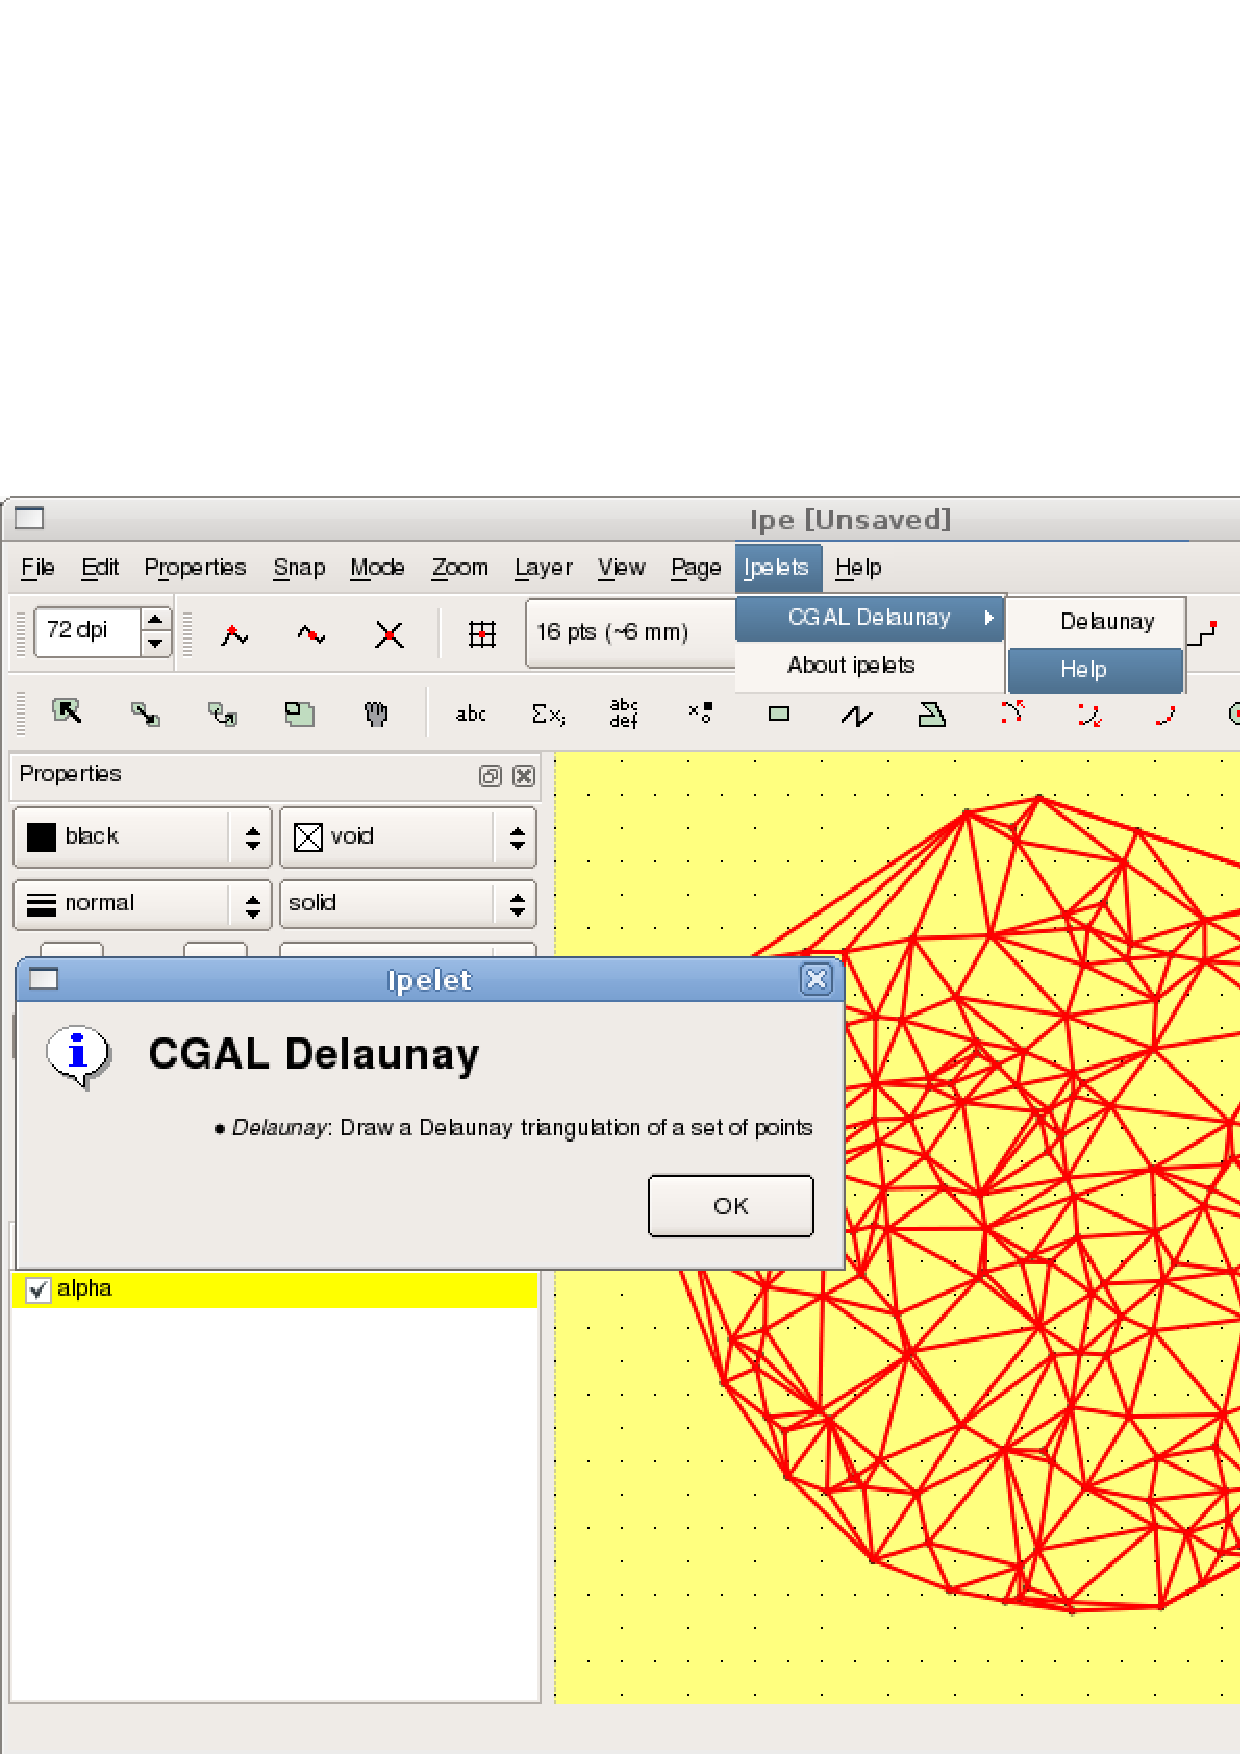
\includegraphics[width=.8\textwidth]{CGAL_ipelets/fig/example}}
    \caption{The ipelet of the example in action.}
  \end{figure}
\end{ccTexOnly}

\begin{ccHtmlOnly}
    <CENTER>
    <A HREF="fig/example.png">
        <img src="fig/example.png" alt="The ipelet of the example in action."></A><P>
    </CENTER>
\end{ccHtmlOnly}


\section{Installation of the Demo Ipelets}
Some working ipelets can be found within
the demo directory of this package. To install them you need
to go to the demo directory of the package and run cmake.
The compilation of these demo requires the source tree and the library of Ipe.
If your Ipe installation is not detected you need to set the cmake
variables \ccc{IPE_INCLUDE_DIR} and \ccc{IPE_LIBRARIES}. If you want
to install ipelets automatically (using \ccc{make install} for example)
you also need to set the cmake variable \ccc{IPELET_INSTALL_DIR}, 
if the ipelet installation path has not already been detected.
These ipelets have been tested with the versions 6.0pre28 to 6.0pre32 of Ipe,
as well as with the version 7 (at least up to version 7.10).
These ipelets are a good starting point to design your own ipelet. For more details on how
to compile an ipelet, please refer to the Ipe manual.



\section{Design and Implementation History}
A first draft of the \cgal{} ipelets has been implemented during the
internship of Nicolas Carrez, in 2005, supervised by Olivier Devillers.
Since then, the ipelets have been rewritten and extended by Sebastien
Loriot as a stand-alone software with the help of Laurent Rineau.
Finally, an enhanced version has been formally contributed to \cgal{} in 2009
by Sebastien Loriot. Sylvain Pion has participated in the discussion
of the overall design, and contributed the Hilbert sort ipelet demo.
